\documentclass{article}

% Required to support mathematical unicode
\usepackage[warnunknown, fasterrors, mathletters]{ucs}
\usepackage[utf8x]{inputenc}

% Always typeset math in display style
\everymath{\displaystyle}

% Use a larger font size
\usepackage[fontsize=14pt]{scrextend}

% Standard mathematical typesetting packages
\usepackage{amsfonts, amsthm, amsmath, amssymb}
\usepackage{mathtools}  % Extension to amsmath

% Symbol and utility packages
\usepackage{cancel, textcomp}
\usepackage[mathscr]{euscript}
\usepackage[nointegrals]{wasysym}

% Extras
\usepackage{physics}  % Lots of useful shortcuts and macros
\usepackage{tikz-cd}  % For drawing commutative diagrams easily
\usepackage{color}  % Add some colour to life
\usepackage{microtype}  % Minature font tweaks
\usepackage[margin=0.5in]{geometry} 
\usepackage{calc}

% Common shortcuts
\def\mbb#1{\mathbb{#1}}
\def\mfk#1{\mathfrak{#1}}

\def\bN{\mbb{N}}
\def\bC{\mbb{C}}
\def\bR{\mbb{R}}
\def\bQ{\mbb{Q}}
\def\bZ{\mbb{Z}}

% Sometimes helpful macros
\newcommand{\func}[3]{#1\colon#2\to#3}
\newcommand{\vfunc}[5]{\func{#1}{#2}{#3},\quad#4\longmapsto#5}
\newcommand{\floor}[1]{\left\lfloor#1\right\rfloor}
\newcommand{\ceil}[1]{\left\lceil#1\right\rceil}
\newcommand{\ti}[1]{\textit{#1}}
\newcommand{\tb}[1]{\textbf{#1}}
\newcommand{\fn}[1]{\footnote{#1}}
% Some standard theorem definitions
\newtheorem{Theorem}{Theorem}
\newtheorem{Proposition}{Theorem}
\newtheorem{Lemma}[Theorem]{Lemma}
\newtheorem{Corollary}[Theorem]{Corollary}

\theoremstyle{definition}
\newtheorem{Definition}[Theorem]{Definition}

\title{\textbf{Logic, Operations and Functions: Essentials}}
\date{\today}
\author{Divya and lastironstar for 18.01 OCW Discord}

\begin{document}
\maketitle
\tableofcontents

\noindent
This is a short set of notes, reviewing the essential concepts of logic, namely, implication of propositions, contrapositives and contradiction. We're doing this mostly so that we can be familiar with the techniques and terminology of how to think about mathematical statements. They have immense importance while trying to think about how to approach proofs. It gives you more things in your mathematical artillery which you can bring up whenever you're in need of mathematical intuition or formal language. 

\section{Propositional Logic}

\Definition{A proposition $p$ is a variable\fn{meaning just a formal expression without any structure} that can take the values true (T or 1) or false (F or 0) and no others}

That's all a proposition is, it's something that can be either true or false. Here goes some more terminology that's related:

\Definition{A proposition which is always true is called a \textit{tautology}, while one which is always false is called a \textit{contradiction}}

\subsection{Unary Operators}
One can build new propositions from given ones by using \textit{logical operators}. The kind of logical operators that give you one proposition from one proposition are called \textit{unary operators} and the ones that take two propositions to give one new proposition are called \textit{binary operators}. There are in total 4 unary operators:
\begin{itemize}
	\item The $\neg$ \textit{negation} operator. E.g P: I am mad has $\neg$P as: I am \textit{not} mad. 
	\item The $\mathrm{id}$ \textit{identity} operator. E.g. P: I am mad has $\mathrm{id}$(P) as: I am mad. And, P': I am not mad has $\mathrm{id}$(P') as: I am not mad. Stays the same. 
	\item The $\top$ \textit{tautology} operation. E.g P: I am mad has $\top_{P}$ as: I am \textit{always} mad. Me being mad is always true. 
	\item The $\perp$ \textit{contradiction} operator. E.g P: I am mad has $\perp_{P}$ as: I am \textit{always not} mad. Me being \textit{not} mad is always true, contradicting P. 
\end{itemize}

These are all the possible ways you can have one proposition from another one.
As an exercise try to fill the entries in this table yourself from your understanding of the unary operators:

\begin{center}
\begin{tabular}{c||c|c|c|c}
	P & $\neg P$ & $\mathrm{id}(P)$ & $\top_{P}$ & $\perp_{P}$ \\
	\hline
	F & - & - & - & - \\
	T & - & - & - & -

\end{tabular}
\end{center}

Also, as a way of practice, write down what each of the unary operations mean in English language while you fill in the above entries. This will help you get used to the concepts of negation, tautology and others while holding your intuition. 

\subsection{Binary Logical Operators}

As defined before, a binary logical operators needs two proposition and then gives you a new proposition by ``operating" on them. And as one can guess by trivial counting, there are 16 such possible operators, we have 4 combinations of the truth values of two propositions and as the binary operator is going to assign two possible truth values to each of those, you'll have 16 in total. We're not going to go into all 16 of them, but just mention a few that are important. Here are those:

\begin{itemize}
	\item The $\land$ \textit{and} operator.
	\item The $\lor$ \textit{or} operator.
	\item The $\implies$ \textit{implies} operator.
	\item The $\iff$ \textit{equivalence} operator.
\end{itemize}

Let's play with these operators for a while and put them in a table. Consider the following two propositions: \\

\noindent
1. $p$: I read books all day. \\
2. $q$: I am mad. \\

Now lets see how the truth tables for each of these binary operators is going to look like for the first two propositions above. I've filled some of the entries, the rest are for you to exercise your muscles of logic. 

\begin{center}
	\begin{tabular}{c||c|c||c|c}
		0 & $p$ & $q$ & $p \land q$ & $p \lor q$ \\
		\hline
		1 & F & F & F & F	\\
		2 & F & T & - & - 	\\	
		3 & T & F & F & -	\\	
		4 & T & T & - & T	\\
		
	\end{tabular}
\end{center}

Here is an explanation in English words for how I filled some of the entries in the above table. 

\vspace{2.5mm}
\textit{\underline{Explanation:}} \\
\vspace{2.5mm}
\noindent

For the first row, what I have is, $p$ and $q$ are both not true. Thus, $q$:I am \textit{not} mad and $p$: I \textit{don't} read books all day. Now to put an entry in the 3rd row of 3rd column, you have to answer the following question: ``\textit{What truth value does $p$ \textbf{and} $q$ together have when $p$ is not true and $q$ is also not true?}" In other words, if me reading books all day is not true and I am not mad, can it be true that I am both mad \textit{and} I read books all day? Notice that the second ``and" in the last question is equivalent to the $\land$ operator on $p$ and $q$. Now, as you can guess the answer to both the questions is NO. If $p$ and $q$ are not true, then $p$ \textit{and} $q$ can't be true, either. 

Now for the next column in the first row, we again have $p$ and $q$ both as false. But this time we'll have to look at $p \lor q$. You ask a similar question like before but replace the \textit{and} with \textit{or}. And you'll find the answer is the same. If $p$ and $q$ are not true, then $p \lor q$ can't be true. 

\vspace{2.5mm}

Easy...heh? Use the same argument and you'll be able to fill all the entries in the table. Now let's get on to the more complicated binary operators, $\implies$ and $\iff$. We consider the same propositions $p$ and $q$ and make another truth table:

\begin{center}
	\begin{tabular}{c||c|c||c|c}
		0 & $p$ & $q$ & $p \implies q$ & $p \iff q$ \\
		\hline
		1 & F & F & T & T\\
		2 & F & T & T & - \\
		3 & T & F & - & - \\
		4 & T & T & T & T \\
	\end{tabular}
\end{center}

\textit{\underline{Explanation:}}

\vspace{2.5mm}

For the first and last row, the entry for $p \iff q $ should be obvious, if you have any of them with different truth values then they're not going to be equivalent. In other words, ``I read books all day" is \textit{equivalent to} ``I am mad" only when both the statements are true or false at the same time. If one of them is true and the other false, you'll lose equivalence. If I read books all day but somehow it turned out that I am not actually mad, then me reading books all day can't be \textit{equivalent} to me being mad. Makes sense? Good, that implies you're not mad!

Next for $p \implies q$ the last row should be trivial. The first row says that if both $p$ and $q$ are not true then what's going to be the truth value for $p \implies q$? You make a similar argument, ``I don't read books all day" ($p$ is false) and ``I am not mad." ($q$ is false) then one can say that ``I read books all day" \textit{implies} ``I am mad". But the interesting thing is even if you make $q$ true keeping $p$ false (2nd row), this doesn't invalidate the implication. This can be surprising at first, that if $p$ is false, no matter what $q$ is, you can have a valid implication that is true. This is also known as ``Ex falso quad libet" meaning ``from a false premise (assumption) anything follows". Think a bit more on this while referring to the table if it isn't immediately clear to you. Try filling the rest of the entries in the table, by making similar arguments but without resorting to self-referential tautology.   

And now I'll put in formal terms what we were trying to do in the lecture. Namely the important use of \textit{contrapositive}. It's going to be obvious after the following theorem and it's explanatory theorem.

\Theorem{Let $p$ and $q$ be propositions. Then $(p \implies q) \iff (\neg q \implies \neg p)$.}

\begin{proof}
	Let's try to understand what the theorem's statement means in the context of our original propositions. It's saying that if $p$ being true implies $q$ being true then that's \textit{equivalent} to saying $q$ being false \textit{implies} $p$ being false. So if ``I read books all day" implies ``I am mad" then it's the same as saying ``I am not mad thus, I don't read books all day."\footnote{This also works in the other direction ($(\neg q \implies \neg p) \implies (p \implies q)$), and in proofs its called the ``if and only if" condition. And when you're faced with such a statement you'll have to prove the statements in both the direction.}

	Now let's try to draw the truth table again, we're going to copy our previous table of $p \implies q$. 
	\begin{center}
		\begin{tabular}{c|c||c|c|c|c}
			$p$ & $q$ & $\neg q$ & $\neg p$ & $p \implies q$ & $(\neg q) \implies (\neg p)$ \\
			\hline
			F & F & T & T & T & T \\
			F & T & F & T & T & - \\
			T & F & T & F & F & F \\
			T & T & F & F & T & - \\
		\end{tabular}
	\end{center}
I'll explain the first and third entries of the last column, but I'd like you to try the others, would be a good exercise of implications among negatives. 

\textit{\underline{Explanation:}} \\
\vspace{2.5mm}

The first entry (of last column) is quite trivial, if both of your propositions--which here are negations--are true, then you can have a valid implication that holds. Translating things again we get, $\neg q$ : I am not mad and $\neg p$ : I don't read books all day, then it's true that me not being mad implies me not reading books all day ($\neg q \implies \neg p$), thus making the contrapositive hold. For the third entry, you have $\neg q$ as true, thus ``I am not mad" and you have $\neg p$ is false, thus ``I am reading books all day". And you have to answer the question, what is the truth value for $\neg q \implies \neg p$ or the statement ``I am not mad implies I am reading books all day", which as you can see can't be true, me reading books all day isn't \textit{necessary} for me being mad\footnote{There have been lunatics who haven't read a word!}. 

When you're done with filling all the entries for last column you'd realise that it's exactly the same as the previous column, and that was entire goal of the proof. Now both the columns and thus the statements are \textit{equivalent}, an implication is equivalent to it's contrapositive. You'd see yourself using this simple-looking statement more than you can think now! 
\end{proof}

\textit{\underline{Remark:}} One can semantically use the $\implies$ in various ways, we mention some of them here, all of them are equivalent to each other: 
\begin{itemize}
	\item  If $p$, then $q$.
	\item $q$ if $p$.
	\item $p$ implies $q$.
	\item $p$ only if $q$.
	\item $p$ is sufficient for $q$.
	\item $q$ is necessary for $p$.
\end{itemize}

\subsection{Functions}

\Definition{A function (or map) $\phi: A \to B$ is a relation such that for each $a \in A$ there exists only one $b \in B$ such that $\phi(a) = b$. Here $A$ is the \textbf{domain} of $\phi$, $B$ is the \textbf{codomain} and $\phi(A) = \{ f(a) : \forall a \in A \} $ is the \textbf{image} of $\phi$.}



\tikzset{every picture/.style={line width=0.75pt}} %set default line width to 0.75pt        

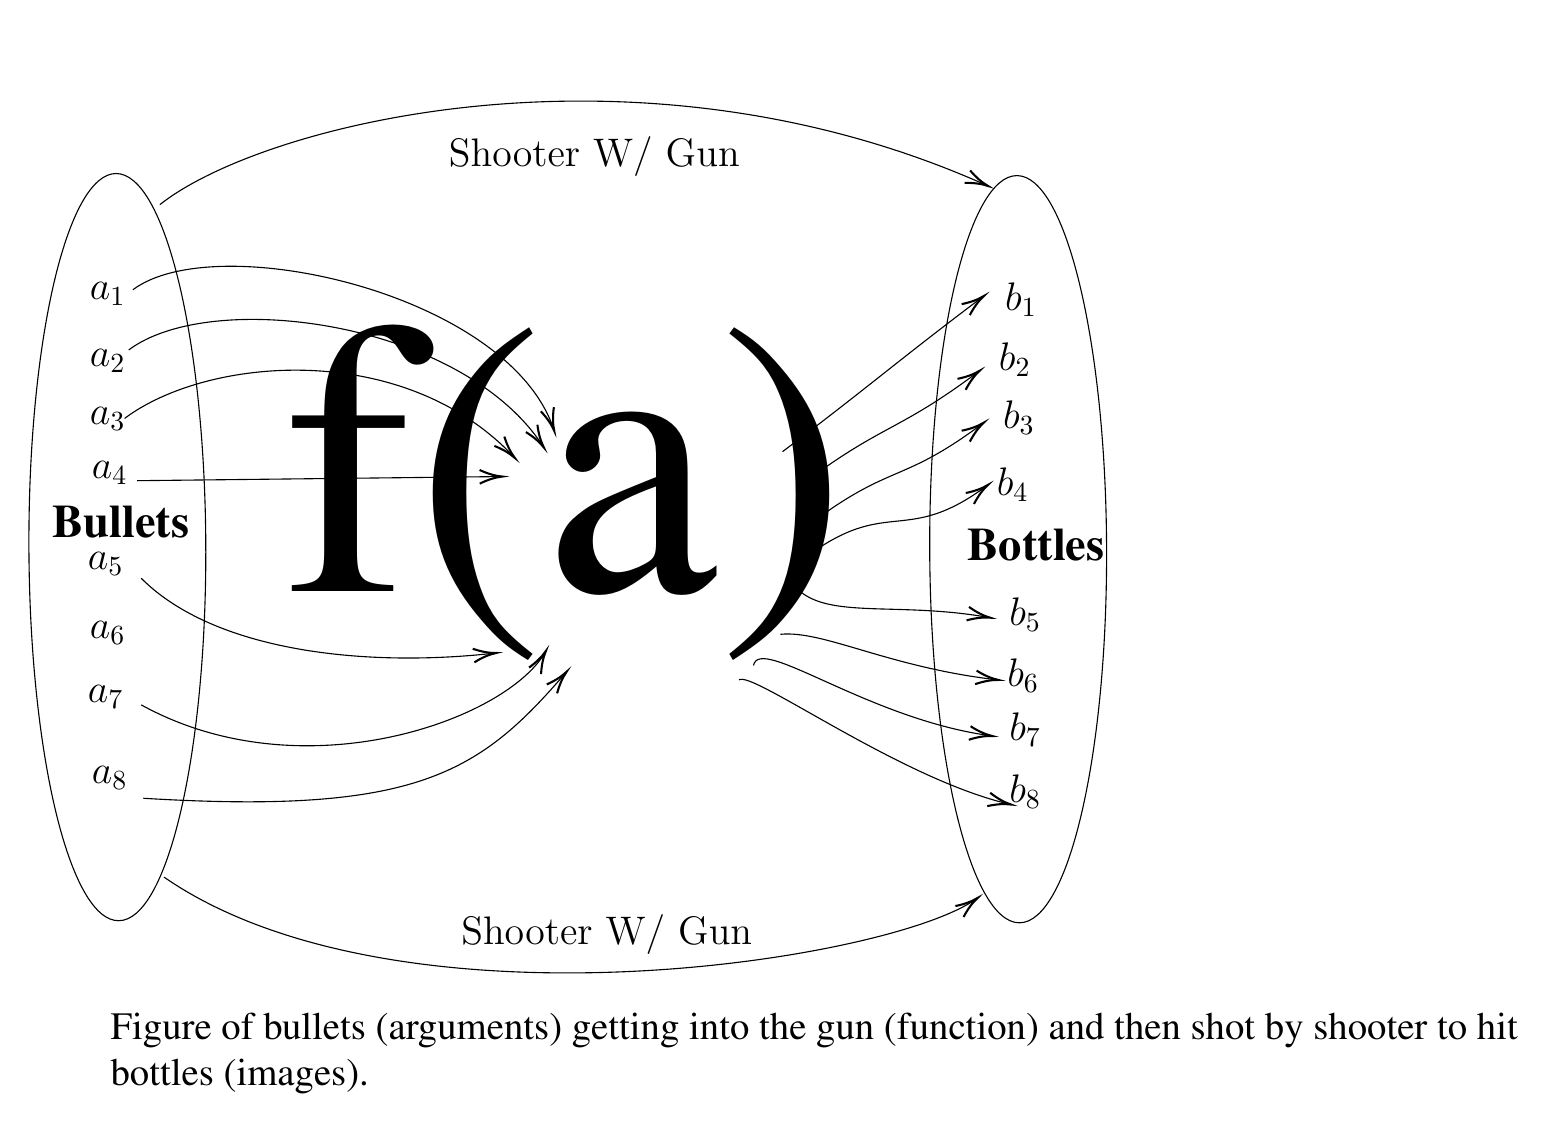
\begin{tikzpicture}[x=0.75pt,y=0.75pt,yscale=-1,xscale=1]
	%uncomment if require: \path (0,526); %set diagram left start at 0, and has height of 526

	%Shape: Ellipse [id:dp5493165154748008] 
	\draw   (87.9,230) .. controls (87.57,130.59) and (106.38,50) .. (129.91,50) .. controls (153.44,50) and (172.79,130.59) .. (173.12,230) .. controls (173.45,329.41) and (154.64,410) .. (131.11,410) .. controls (107.57,410) and (88.23,329.41) .. (87.9,230) -- cycle ;
	%Shape: Ellipse [id:dp8348182556077381] 
	\draw   (521.9,231) .. controls (521.57,131.59) and (540.38,51) .. (563.91,51) .. controls (587.44,51) and (606.79,131.59) .. (607.12,231) .. controls (607.45,330.41) and (588.64,411) .. (565.11,411) .. controls (541.57,411) and (522.23,330.41) .. (521.9,231) -- cycle ;
	%Curve Lines [id:da6045410144044325] 
	\draw    (151,65) .. controls (200,26) and (381,-20) .. (550,56) ;
	\draw [shift={(550,56)}, rotate = 204.21] [color={rgb, 255:red, 0; green, 0; blue, 0 }  ][line width=0.75]    (10.93,-3.29) .. controls (6.95,-1.4) and (3.31,-0.3) .. (0,0) .. controls (3.31,0.3) and (6.95,1.4) .. (10.93,3.29)   ;
	%Curve Lines [id:da5975543785444846] 
	\draw    (153,389) .. controls (264.87,466.22) and (500.23,429.75) .. (543.74,399.9) ;
	\draw [shift={(545,399)}, rotate = 503.13] [color={rgb, 255:red, 0; green, 0; blue, 0 }  ][line width=0.75]    (10.93,-3.29) .. controls (6.95,-1.4) and (3.31,-0.3) .. (0,0) .. controls (3.31,0.3) and (6.95,1.4) .. (10.93,3.29)   ;
	%Curve Lines [id:da4111327650952241] 
	\draw    (138,106) .. controls (177.8,76.15) and (318.58,107.68) .. (340.68,173.01) ;
	\draw [shift={(341,174)}, rotate = 252.35] [color={rgb, 255:red, 0; green, 0; blue, 0 }  ][line width=0.75]    (10.93,-3.29) .. controls (6.95,-1.4) and (3.31,-0.3) .. (0,0) .. controls (3.31,0.3) and (6.95,1.4) .. (10.93,3.29)   ;
	%Curve Lines [id:da6364954933005966] 
	\draw    (136,135) .. controls (175.8,105.15) and (295.79,120.84) .. (335.41,181.09) ;
	\draw [shift={(336,182)}, rotate = 237.41] [color={rgb, 255:red, 0; green, 0; blue, 0 }  ][line width=0.75]    (10.93,-3.29) .. controls (6.95,-1.4) and (3.31,-0.3) .. (0,0) .. controls (3.31,0.3) and (6.95,1.4) .. (10.93,3.29)   ;
	%Curve Lines [id:da5118080900884339] 
	\draw    (134,168) .. controls (173.8,138.15) and (268.05,130.08) .. (321.2,186.15) ;
	\draw [shift={(322,187)}, rotate = 227.07999999999998] [color={rgb, 255:red, 0; green, 0; blue, 0 }  ][line width=0.75]    (10.93,-3.29) .. controls (6.95,-1.4) and (3.31,-0.3) .. (0,0) .. controls (3.31,0.3) and (6.95,1.4) .. (10.93,3.29)   ;
	%Straight Lines [id:da4127986459387216] 
	\draw    (140,198) -- (189.98,197.43) -- (314,196.02) ;
	\draw [shift={(316,196)}, rotate = 539.35] [color={rgb, 255:red, 0; green, 0; blue, 0 }  ][line width=0.75]    (10.93,-3.29) .. controls (6.95,-1.4) and (3.31,-0.3) .. (0,0) .. controls (3.31,0.3) and (6.95,1.4) .. (10.93,3.29)   ;
	%Curve Lines [id:da5243034902699031] 
	\draw    (142,245) .. controls (177.64,280.64) and (250.52,287.86) .. (311.17,281.21) ;
	\draw [shift={(313,281)}, rotate = 533.45] [color={rgb, 255:red, 0; green, 0; blue, 0 }  ][line width=0.75]    (10.93,-3.29) .. controls (6.95,-1.4) and (3.31,-0.3) .. (0,0) .. controls (3.31,0.3) and (6.95,1.4) .. (10.93,3.29)   ;
	%Curve Lines [id:da3091052238986527] 
	\draw    (142,306) .. controls (218.83,348.36) and (316.03,314.06) .. (336.14,281.49) ;
	\draw [shift={(337,280)}, rotate = 478.61] [color={rgb, 255:red, 0; green, 0; blue, 0 }  ][line width=0.75]    (10.93,-3.29) .. controls (6.95,-1.4) and (3.31,-0.3) .. (0,0) .. controls (3.31,0.3) and (6.95,1.4) .. (10.93,3.29)   ;
	%Curve Lines [id:da9993769861517163] 
	\draw    (143,351) .. controls (273.68,358.92) and (304.39,339.4) .. (345.74,291.46) ;
	\draw [shift={(347,290)}, rotate = 490.6] [color={rgb, 255:red, 0; green, 0; blue, 0 }  ][line width=0.75]    (10.93,-3.29) .. controls (6.95,-1.4) and (3.31,-0.3) .. (0,0) .. controls (3.31,0.3) and (6.95,1.4) .. (10.93,3.29)   ;
	%Curve Lines [id:da15707957328772904] 
	\draw    (451,184) .. controls (490.6,154.3) and (507.66,139.3) .. (546.81,109.9) ;
	\draw [shift={(548,109)}, rotate = 503.13] [color={rgb, 255:red, 0; green, 0; blue, 0 }  ][line width=0.75]    (10.93,-3.29) .. controls (6.95,-1.4) and (3.31,-0.3) .. (0,0) .. controls (3.31,0.3) and (6.95,1.4) .. (10.93,3.29)   ;
	%Curve Lines [id:da5778226515665781] 
	\draw    (460,200) .. controls (499.6,170.3) and (505.88,174.9) .. (544.81,145.89) ;
	\draw [shift={(546,145)}, rotate = 503.13] [color={rgb, 255:red, 0; green, 0; blue, 0 }  ][line width=0.75]    (10.93,-3.29) .. controls (6.95,-1.4) and (3.31,-0.3) .. (0,0) .. controls (3.31,0.3) and (6.95,1.4) .. (10.93,3.29)   ;
	%Curve Lines [id:da03160935359492267] 
	\draw    (464,219) .. controls (503.6,189.3) and (507.92,199.78) .. (546.81,170.89) ;
	\draw [shift={(548,170)}, rotate = 503.13] [color={rgb, 255:red, 0; green, 0; blue, 0 }  ][line width=0.75]    (10.93,-3.29) .. controls (6.95,-1.4) and (3.31,-0.3) .. (0,0) .. controls (3.31,0.3) and (6.95,1.4) .. (10.93,3.29)   ;
	%Curve Lines [id:da6168903053757182] 
	\draw    (462,235) .. controls (501.6,205.3) and (509.84,229.51) .. (548.81,200.88) ;
	\draw [shift={(550,200)}, rotate = 503.13] [color={rgb, 255:red, 0; green, 0; blue, 0 }  ][line width=0.75]    (10.93,-3.29) .. controls (6.95,-1.4) and (3.31,-0.3) .. (0,0) .. controls (3.31,0.3) and (6.95,1.4) .. (10.93,3.29)   ;
	%Curve Lines [id:da08728689492086161] 
	\draw    (458,250) .. controls (472.85,264.85) and (506.32,256.18) .. (549.68,263.77) ;
	\draw [shift={(551,264)}, rotate = 190.3] [color={rgb, 255:red, 0; green, 0; blue, 0 }  ][line width=0.75]    (10.93,-3.29) .. controls (6.95,-1.4) and (3.31,-0.3) .. (0,0) .. controls (3.31,0.3) and (6.95,1.4) .. (10.93,3.29)   ;
	%Curve Lines [id:da3916175512343014] 
	\draw    (450,272) .. controls (470.79,270.02) and (501.38,287.64) .. (553.42,293.82) ;
	\draw [shift={(555,294)}, rotate = 186.46] [color={rgb, 255:red, 0; green, 0; blue, 0 }  ][line width=0.75]    (10.93,-3.29) .. controls (6.95,-1.4) and (3.31,-0.3) .. (0,0) .. controls (3.31,0.3) and (6.95,1.4) .. (10.93,3.29)   ;
	%Curve Lines [id:da04095416179837441] 
	\draw    (437,287) .. controls (439.97,272.15) and (490.96,312.19) .. (550.2,320.75) ;
	\draw [shift={(552,321)}, rotate = 187.59] [color={rgb, 255:red, 0; green, 0; blue, 0 }  ][line width=0.75]    (10.93,-3.29) .. controls (6.95,-1.4) and (3.31,-0.3) .. (0,0) .. controls (3.31,0.3) and (6.95,1.4) .. (10.93,3.29)   ;
	%Curve Lines [id:da7424189877659317] 
	\draw    (430,294) .. controls (435.94,289.05) and (506.57,340.95) .. (559.4,353.63) ;
	\draw [shift={(561,354)}, rotate = 192.76] [color={rgb, 255:red, 0; green, 0; blue, 0 }  ][line width=0.75]    (10.93,-3.29) .. controls (6.95,-1.4) and (3.31,-0.3) .. (0,0) .. controls (3.31,0.3) and (6.95,1.4) .. (10.93,3.29)   ;

	% Text Node
	\draw (98,209) node [anchor=north west][inner sep=0.75pt]   [align=left] {\textbf{{\fontfamily{ptm}\selectfont {\large Bullets}}}};
	% Text Node
	\draw (116,101.4) node [anchor=north west][inner sep=0.75pt]    {$a_{1}$};
	% Text Node
	\draw (116,133.4) node [anchor=north west][inner sep=0.75pt]    {$a_{2}$};
	% Text Node
	\draw (117,187.4) node [anchor=north west][inner sep=0.75pt]    {$a_{4}$};
	% Text Node
	\draw (116,161.4) node [anchor=north west][inner sep=0.75pt]    {$a_{3}$};
	% Text Node
	\draw (115,231.4) node [anchor=north west][inner sep=0.75pt]    {$a_{5}$};
	% Text Node
	\draw (116,264.4) node [anchor=north west][inner sep=0.75pt]    {$a_{6}$};
	% Text Node
	\draw (115,295.4) node [anchor=north west][inner sep=0.75pt]    {$a_{7}$};
	% Text Node
	\draw (117,334.4) node [anchor=north west][inner sep=0.75pt]    {$a_{8}$};
	% Text Node
	\draw (557,101.4) node [anchor=north west][inner sep=0.75pt]    {$b_{1}$};
	% Text Node
	\draw (554,130.4) node [anchor=north west][inner sep=0.75pt]    {$b_{2}$};
	% Text Node
	\draw (556,158.4) node [anchor=north west][inner sep=0.75pt]    {$b_{3}$};
	% Text Node
	\draw (553,190.4) node [anchor=north west][inner sep=0.75pt]    {$b_{4}$};
	% Text Node
	\draw (559,253.4) node [anchor=north west][inner sep=0.75pt]    {$b_{5}$};
	% Text Node
	\draw (558,282.4) node [anchor=north west][inner sep=0.75pt]    {$b_{6}$};
	% Text Node
	\draw (559,308.4) node [anchor=north west][inner sep=0.75pt]    {$b_{7}$};
	% Text Node
	\draw (559,338.4) node [anchor=north west][inner sep=0.75pt]    {$b_{8}$};
	% Text Node
	\draw (539,220) node [anchor=north west][inner sep=0.75pt]   [align=left] {\textbf{{\large {\fontfamily{ptm}\selectfont Bottles}}}};
	% Text Node
	\draw (289,31) node [anchor=north west][inner sep=0.75pt]   [align=left] {Shooter W/ Gun};
	% Text Node
	\draw (295,406) node [anchor=north west][inner sep=0.75pt]   [align=left] {Shooter W/ Gun};
	% Text Node
	\draw (210,122) node [anchor=north west][inner sep=0.75pt]  [font=\fontsize{10em}{12em}\selectfont] [align=left] {{\fontfamily{ptm}\selectfont f(a)}};
	% Text Node
	\draw (126,453) node [anchor=north west][inner sep=0.75pt]   [align=left] {{\fontfamily{ptm}\selectfont Figure of bullets (arguments) getting into the gun (function) and then shot by shooter to hit}\\{\fontfamily{ptm}\selectfont bottles (images). }};


\end{tikzpicture}

\vspace{5mm}

Consider a function to be like a gun (more like a pistol), the bullets in the gun to be elements in the domain, and coke bottles as elements in the codomain. So what our gun does is it hits a coke bottle with one bullet, the set of all coke bottles that got hit by all the bullets we fired is the image of our function. It's everything that got hit. 

Now lets use this analogy to define injectivity and surjectivity. Consider that while shooting, we make it entirely sure that one bullet that gets fired from my gun hits \textit{only one} bottle. So if I found bottles $b_{1}$ and $b_{2}$ were hit by the same gun, then I'm sure that those two bottles are one and the same.\footnote{Mathematically it means $f(x) = f(x') \implies x =x'$.}Such a gun is defined as \textit{\textbf{injective}}, if two bottles got hit, then there \emph{must} be two bullets that got fired. Do you see the problem with such a gun shooter? Its that if he follows this, he might not be able to shoot all bottles we have in the codomain. As, if the number of bullets is less than the number of bottles and he hits exactly one bottle with one bullet, then obviously he's going to miss a bunch of bottles. 


Now consider another case, you have another shooter who uses the gun in such a manner that he \emph{always} hits every bottle in the codomain. After a session of shooting, you're going to find that every bottle was hit and is broken. This is the case of a \textit{\textbf{surjective function}}, no matter what bottle we consider we're always going to find \emph{at least} one bullet that hit it.\footnote{Mathematically, it means the whole image of the function is the codomain itself. So $\mathrm{im}_{\phi}(A) = B$} Can you see the problem with this shooter? He surely is able to hit every single bottle, but he probably has tried more than one bullet on some bottles out of which some got missed and only of them hit the bottle. In this case you can actually imagine the shooter having a double-barrel gun or something that can shoot more than one bullets at a time because we need \emph{at least} one bullet to hit, but we can go for more! Thus this shooter is wasting those precious bullets!

So who's the \textit{perfect} shooter? As some of you might have guessed, it'd be the shooter who has the ability to hit a bottle \emph{exactly} with one bullet and has enough bullets to hit \emph{each and every} bottle in the codomain. It's trivial to point out that this is a "special" shooter, he's actually the \emph{nicest} of all shooters we can get. In mathematics we call such shooters (more like, functions!) \textit{\textbf{bijective}}, every bullet hits only one bottle and all bottles get hit\footnote{Mathematically you say it as a one-to-one correspondence, you have exactly one unique ordered pair of $(x,f(x))$ in each case.}As you might've already guessed, this special shooter has the skills of both the other two shooters we hired, and thus a bijective function is one which is both injective and surjective.

Graphically, you imagine a function to intersect (or more like, hit!) the graph at precisely one point, for it to be injective. And similarly for surjective you need the function's image to be the graph itself (``everything gets hit"). 
\\
\\
This is all we covered on September 13rd, join us tomorrow at 2PM UTC to continue our journey through logic, functions, trigonometry and finally into Calculus! 















\end{document}
